\documentclass{article}

\usepackage[final]{neurips_2019}
\usepackage[utf8]{inputenc}
\usepackage[T1]{fontenc}
\usepackage{hyperref}
\usepackage{url}
\usepackage{booktabs}
\usepackage{amsfonts}
\usepackage{amsmath}
\usepackage{microtype}
\usepackage{graphicx}
\usepackage{xcolor}
\usepackage{caption}
\usepackage{subcaption}
\usepackage{enumitem}
\geometry{left=1.5cm, right=1.5cm}

\title{
  Multitask BERT for Student Support Understanding \\
  \vspace{0.15cm}
  \large \normalfont Natural Language Processing Course Project
}

\author{
  Vu Thuong Tin \\
  Hanoi University of Science and Technology \\
  \And
  Chu Anh Duc \\
  Hanoi University of Science and Technology \\
  \And
  Tran Quang Hung \\
  Hanoi University of Science and Technology \\
  \And
  Nguyen Xuan Khai \\
  Hanoi University of Science and Technology \\
  \And
  Do Dang Vu \\
  Hanoi University of Science and Technology
}

\begin{document}

\maketitle
\vspace{-0.4cm}

\begin{abstract}
This project presents a fully self-implemented multitask BERT system for three related natural language understanding tasks: sentiment analysis, paraphrase detection, and semantic textual similarity. The main engineering contribution is that we re-coded the BERT encoder ourselves instead of calling a ready-made Transformer model during the forward pass. Our implementation reproduces HuggingFace BERT with a maximum hidden-state difference of only $4.29\times10^{-6}$, showing that the custom encoder is numerically faithful. After multitask fine-tuning, our best self-implemented model reaches 0.520 SST accuracy, 0.864 Quora paraphrase accuracy, and 0.785 STS Pearson correlation, with an aggregate score of 0.759. This is nearly tied with the HuggingFace-backed baseline score of 0.761, despite using our own encoder implementation. We also evaluate optimizer and schedule choices, including AdamW, Muon, constant learning rate, and linear warmup/decay. The final model uses AdamW with linear warmup and decay because it clearly preserves the pretrained model better than Muon. Finally, we build two demos: a direct checkpoint inference demo for the three benchmark tasks, and a product-style Smart Student Support Assistant that maps the same model to a concrete use case.
\end{abstract}

\vspace{-0.5cm}

\section{Introduction}

Modern student support systems need to process many short, noisy, and semantically related text requests. A student may ask whether two regulations mean the same thing, search for the closest entry in a handbook, or send a frustrated message that should be handled with higher priority. These use cases are different at the surface level, but they share a common requirement: the system must represent sentence meaning well.

We approach this problem through multitask fine-tuning of BERT \cite{devlin2019bert}. One encoder is shared across three tasks: Stanford Sentiment Treebank (SST) sentiment classification, Quora duplicate question detection, and Semantic Textual Similarity Benchmark (STS-B) regression. The training objective encourages the encoder to preserve information that is useful across single-sentence classification and sentence-pair matching.

The project started from the same modeling direction as the previous Multitask BERT report, but the codebase was rebuilt around a stronger requirement: the BERT encoder itself must be implemented by our team. The encoder forward pass no longer delegates to \texttt{transformers.AutoModel}; it implements embedding lookup, multi-head self-attention, feed-forward blocks, residual connections, layer normalization, and pooler logic directly. HuggingFace remains useful for tokenizer and weight compatibility, but the model path used for the main result is our own PyTorch implementation. The parity check is a central result: our custom encoder differs from the reference backend by only $4.29\times10^{-6}$ on the final hidden states, and its final aggregate score of 0.759 is almost the same as the ready-made-library baseline score of 0.761.

\section{Related Work}

BERT introduced bidirectional Transformer pretraining with masked language modeling and next sentence prediction \cite{devlin2019bert}. Fine-tuning BERT on downstream tasks is a strong baseline, but single-task fine-tuning can be unstable on small datasets and may not exploit relationships between tasks. Multitask learning addresses this by sharing representations across related objectives \cite{caruana1997multitask}. MT-DNN showed that a shared pretrained encoder with task-specific heads can perform well across many natural language understanding tasks \cite{liu2019mtdnn}.

For sentence-pair tasks, Sentence-BERT popularized simple and effective pair features such as concatenation, absolute difference, and cosine similarity over sentence embeddings \cite{reimers2019sbert}. Our paraphrase and STS heads use this idea, and the rich relational layer shares an intermediate representation between these two tasks because both measure semantic closeness.

We also experimented with optimizer and schedule choices. AdamW is the standard fine-tuning optimizer for BERT-like models \cite{loshchilov2019adamw}. Muon was tested as an alternative optimizer, but in our experiments it did not outperform AdamW under the available compute budget. Linear warmup and decay provided the best self-implemented result.

\section{Methodology}

\subsection{Task Formulation}

The model receives either one sentence or a pair of sentences and outputs one of three task predictions.

\textbf{SST sentiment analysis.} Given a sentence, the model predicts one of five sentiment classes. We optimize cross-entropy loss and report accuracy.

\textbf{Quora paraphrase detection.} Given two questions, the model predicts whether they are duplicates. We optimize binary cross-entropy loss and report accuracy.

\textbf{STS semantic similarity.} Given two sentences, the model predicts a real-valued similarity score in the range $[0,5]$. We optimize mean squared error and report Pearson correlation.

For comparison across tasks, we use the aggregate score
\[
S = \frac{\text{SST}_{acc} + \text{Para}_{acc} + (\text{STS}_{r}+1)/2}{3}.
\]
The STS correlation is normalized from $[-1,1]$ to $[0,1]$ before averaging.

\subsection{BERT Architecture}

BERT is built from a stack of Transformer encoder layers. Each input sentence is first converted into WordPiece token ids. For every token, BERT sums three embeddings: token embedding, positional embedding, and segment embedding. Segment embeddings distinguish sentence A from sentence B in pairwise tasks such as paraphrase detection and semantic similarity.

The embedded sequence is processed by repeated Transformer encoder blocks. Each block has a multi-head self-attention module followed by a position-wise feed-forward network. Residual connections and layer normalization are applied around both sublayers. Multi-head attention allows the model to attend to multiple relation patterns in the same sentence, such as local syntax, long-range dependencies, and cross-sentence alignment. After the final encoder layer, the hidden state of the \texttt{[CLS]} token is used as a pooled sentence representation for classification and regression heads.

This architecture is a good fit for our project because all three tasks require contextual sentence understanding. SST needs a representation of sentence-level sentiment, while Quora and STS need representations that preserve semantic equivalence between sentence pairs.

\subsection{Self-Implemented BERT Encoder}

The main encoder is implemented in \texttt{src/multitask\_bert/models/bert\_encoder.py}. It follows the BERT-base architecture and loads pretrained \texttt{bert-base-uncased} weights into our own modules. The implementation covers token, position, and segment embeddings; scaled dot-product multi-head attention; Transformer feed-forward blocks; residual paths; layer normalization; dropout; and the pooled \texttt{[CLS]} representation.

To verify correctness, we compared the self-implemented encoder against a HuggingFace backend using the same inputs and weights. The maximum difference in the final hidden state was approximately $4.29 \times 10^{-6}$ and the maximum difference in the pooler output was approximately $9.54 \times 10^{-7}$. This confirms that the implementation is numerically aligned with the reference backend before fine-tuning.

\subsection{Multitask Architecture}

The shared encoder produces sentence representations. The task heads are intentionally lightweight so that most learning pressure remains on the shared representation.

For SST, we pass the pooled \texttt{[CLS]} representation into a linear classifier. For paraphrase detection, we encode both sentences and build pair features from $h_u$, $h_v$, and $|h_u-h_v|$. For STS, we use pairwise representation features and regress to a scalar similarity score. The rich relational variant adds a shared hidden layer for the paraphrase and STS branches because both tasks compare sentence pairs. This gives the smaller STS dataset access to representation patterns learned from the larger Quora duplicate-question dataset.

\subsection{Rich Relational Layer}

The relational layer is motivated by the observation that paraphrase detection and semantic textual similarity are not independent tasks. Both require deciding whether two sentences express related meanings. However, they differ in output format: paraphrase detection is a binary classification task, while STS is a graded regression task. We therefore avoid fully sharing the output head, but share an intermediate representation.

Given two pooled sentence vectors $h_u$ and $h_v$, the relational layer receives a normalized element-wise interaction:
\[
z = \frac{h_u \odot h_v}{\|h_u\|_2\|h_v\|_2+\epsilon}.
\]
This vector is passed through a learned projection and nonlinearity before branching into the paraphrase and STS heads. Compared with raw cosine similarity, this keeps dimension-wise interaction information and gives the model a trainable path for learning which semantic dimensions matter for sentence-pair decisions.

\subsection{Training Strategy and Task Sampling}

The framework supports round-robin and interleaved training. Round-robin training cycles through SST, Quora, and STS batches so that every optimization window sees all tasks. Interleaved training allows task-specific batch sizes, which is useful because Quora is much larger than SST and STS. The best reported model uses the self-implemented encoder, interleaved multitask training, AdamW, weight decay of 0.01, learning rate $2\times 10^{-5}$, 20 epochs, and linear warmup/decay with warmup ratio 0.1.

The interleaved setup uses task-specific batch sizes: SST uses a small batch, STS uses a small batch, and Quora uses a much larger batch. This approximates the dataset imbalance without allowing the Quora task to completely dominate each epoch. The training loop evaluates the dev sets after every epoch and stores the checkpoint with the best aggregate score.

\subsection{Optimizer Choices}

AdamW is the main optimizer. It decouples weight decay from the adaptive gradient update and is the conventional choice for BERT fine-tuning. We use standard no-decay groups for biases and layer-normalization parameters.

Muon was tested as an alternative optimizer. Our implementation applies Muon only to hidden two-dimensional encoder matrices and keeps embeddings, heads, biases, pooler, and normalization parameters on Adam-style updates. This split is intentional: Muon is designed for matrix-shaped hidden layers, while applying it indiscriminately to all parameters would be inappropriate for BERT fine-tuning.

Despite this guarded setup, Muon was worse than AdamW. The high-learning-rate Muon run damaged the pretrained representation almost immediately, with aggregate scores around 0.46--0.52 in the early epochs. The conservative Muon configuration was less destructive, but it still reached only 0.750 aggregate, below the 0.759 AdamW result. The conclusion is direct: for this BERT fine-tuning setting, AdamW is the better optimizer. Muon's orthogonalized matrix updates disturb pretrained weights too strongly, and the model loses useful sentence-pair geometry for Para and STS.

\section{Experiments}

\subsection{Datasets}

We use the same three benchmark tasks as the earlier Multitask BERT work. SST-5 is a five-class sentence sentiment dataset. Quora Question Pairs is a binary duplicate-question dataset. STS-B is a sentence-pair semantic similarity dataset with real-valued labels. The training code tokenizes text with a BERT-compatible tokenizer, pads sequences, and creates task-specific dataloaders through a common data registry.

\subsection{Experimental Setup}

All main experiments use the \texttt{bert-base-uncased} tokenizer and pretrained weights. The best self-implemented run is stored as:
\begin{center}
\small
\texttt{runs/report\_best\_self\_impl\_20e\_linear\_warmup\_lr2e5/best.pt}
\end{center}

We ran multiple ablations over optimizer, learning-rate schedule, task emphasis, and backend choice. The HuggingFace backend is not treated as the main submission because the project goal is to keep the model implementation under our control. It is included as an upper-bound and parity check.

\begin{table}[h]
\centering
\caption{Main training configurations considered during development.}
\begin{tabular}{p{0.24\textwidth}p{0.28\textwidth}p{0.35\textwidth}}
\toprule
Configuration & Purpose & Outcome \\
\midrule
AdamW, constant LR & Establish self-implemented baseline & Stable but below scheduled runs. \\
AdamW, linear warmup/decay & Test standard BERT fine-tuning schedule & Best self-implemented aggregate score. \\
AdamW, cosine warmup/decay & Alternative schedule & Worse than linear schedule in this setting. \\
Muon + auxiliary Adam & Test optimizer alternative & Unstable at high LR; conservative setting still below AdamW. \\
HF backend & Sanity check reference implementation & Slightly higher aggregate, confirms self-implementation is close. \\
\bottomrule
\end{tabular}
\label{tab:configs}
\end{table}

\subsection{Results}

\begin{table}[h]
\centering
\caption{Development results for the main self-implemented model and important ablations.}
\begin{tabular}{lcccc}
\toprule
Model / setting & SST Acc. & Para Acc. & STS Pearson & Aggregate \\
\midrule
Self-impl, AdamW, 20e, linear warmup, lr $2e^{-5}$ & \textbf{0.520} & \textbf{0.864} & 0.785 & \textbf{0.759} \\
HF backend sanity baseline, 10e & 0.526 & 0.861 & \textbf{0.790} & 0.761 \\
Self-impl, AdamW, 20e, no schedule & 0.505 & 0.860 & 0.784 & 0.752 \\
Self-impl, Muon, 20e, fine-tune safe & 0.523 & 0.851 & 0.750 & 0.750 \\
Self-impl, Muon, high LR early run & 0.262 & 0.720 & 0.145 & 0.518 \\
\bottomrule
\end{tabular}
\label{tab:main-results}
\end{table}

The strongest self-implemented run reaches an aggregate score of 0.759. Its paraphrase score is close to the previous report's best Quora result, and its SST score is higher than the previously reported rich-relational configuration. STS remains the hardest metric to match: the earlier report reached approximately 0.808 Pearson with rich relational training, while our best self-implemented result reaches 0.785. Since the encoder parity check is extremely tight, this lower STS score should be investigated through concrete prediction errors rather than explained away as an implementation failure.

\begin{figure}[h]
\centering
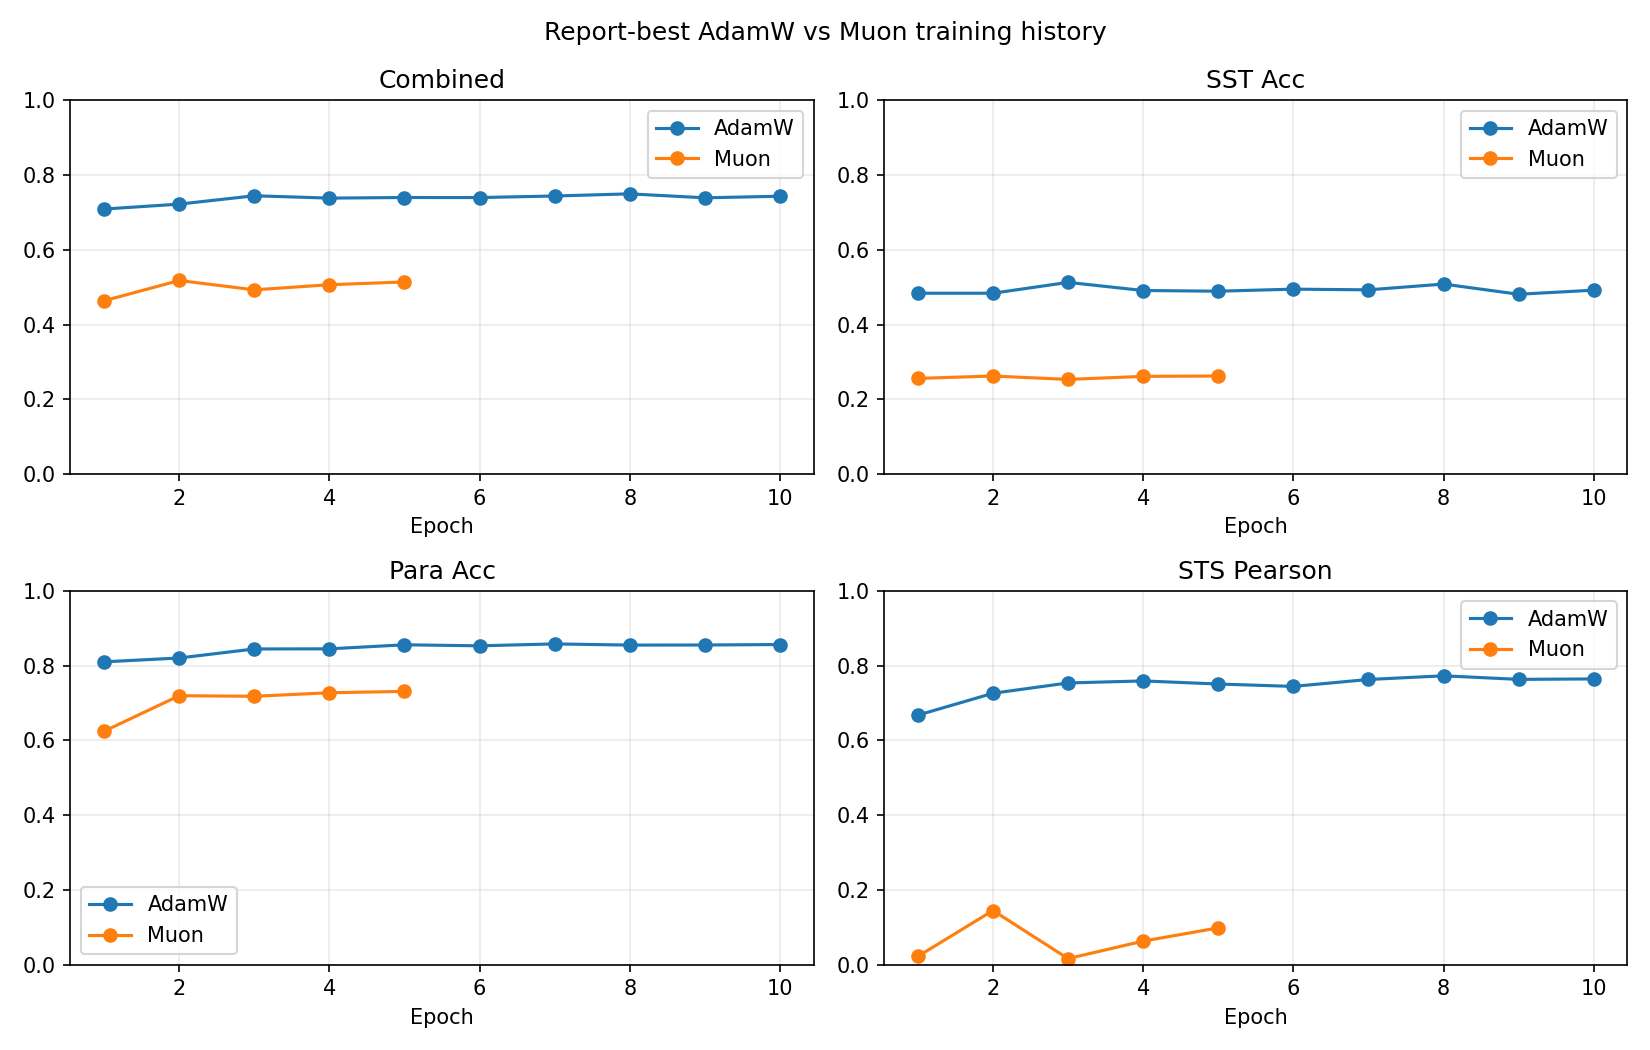
\includegraphics[width=0.72\textwidth]{figures/adamw_vs_muon_history.png}
\caption{Training history comparison between AdamW and Muon experiments. AdamW gives a stronger and more stable final aggregate score in our current setup.}
\label{fig:history}
\end{figure}

\subsection{Scheduler Analysis}

The HuggingFace-backed run is slightly better than the self-implemented model, but the margin is small: 0.761 versus 0.759 aggregate. Because the pretrained forward pass matches numerically before fine-tuning, this difference is acceptable for a self-implementation project. It also shows that the current framework can reproduce the behavior of a standard BERT stack closely enough to support meaningful ablations.

Linear warmup and decay improved the self-implemented model more than a constant learning rate. This matches common BERT fine-tuning practice: warmup reduces the risk of damaging pretrained weights early in training, while decay helps the model settle into a better validation region after the task heads have adapted.

\subsection{Optimizer Analysis: AdamW Beats Muon}

Muon did not improve the final model. The unsafe high-LR run is clearly not competitive: SST remains close to a weak majority-class behavior, STS correlation is very low, and the aggregate score peaks near 0.518. This means Muon was not merely slower; it corrupted the pretrained representation and pushed the model into a poor region for multitask fine-tuning.

The fine-tuning-safe Muon run is more informative. It preserves SST accuracy reasonably well, but Para and STS decrease. This pattern shows that Muon hurts the shared sentence-pair geometry learned by pretrained BERT. Para and STS depend heavily on that geometry, so damaging it lowers duplicate-question accuracy and similarity correlation. AdamW is clearly better here because its adaptive per-parameter updates make smaller, safer changes to the pretrained weights.

Another practical issue is that Muon introduces more hyperparameters: matrix selection, Muon learning rate, momentum, Newton-Schulz steps, Nesterov choice, and auxiliary Adam settings. The extra complexity did not buy better performance. Our final decision is therefore simple: use AdamW, not Muon, for this project.

\subsection{Error Analysis}

The STS score of 0.785 is the main remaining weakness of the system. This number is still usable, but it is lower than the paraphrase score and lower than the best STS number reported in the earlier project. The next step is to inspect actual sentence pairs where the model prediction differs strongly from the gold similarity label.

\begin{center}
\fbox{\begin{minipage}{0.92\textwidth}
\textbf{To be completed before final submission.} Insert 2--3 concrete STS error examples here. For each example, include: sentence A, sentence B, gold STS score, predicted STS score, absolute error, and a short explanation of why the pair is difficult. Good examples should show different failure types, such as lexical overlap with different meaning, low lexical overlap with similar meaning, or numerical/entity mismatch.
\end{minipage}}
\end{center}

This manual error analysis should make the STS discussion evidence-based. Instead of giving a generic explanation, the report should point to real prediction failures and use them to explain which semantic patterns the model still misses.

\section{Demo Application}

To make the model easier to evaluate and present, we built two demos.

\textbf{Checkpoint inference demo.} The first demo directly loads one checkpoint and exposes three independent inference modes: SST sentiment classification, Quora-style paraphrase detection, and STS similarity scoring. This demo is useful for verifying that the trained model can be loaded and queried without running the training pipeline.

\textbf{Smart Student Support Assistant.} The second demo maps the same checkpoint to a product-oriented workflow:

\begin{itemize}
    \item SST predicts whether a student message sounds negative, neutral, or positive. This can help prioritize frustrated requests.
    \item Paraphrase detection checks whether a new question duplicates an existing FAQ.
    \item STS ranks handbook entries or support documents by semantic relevance to a student query.
\end{itemize}

The demo includes a small English subset of a HUST student handbook converted into CSV format. Uploading a real document set is optional: without upload, the demo uses the built-in subset; with upload, it can rank custom rows that contain title, question, answer, or content fields. This use case is intentionally simple, but it gives the three benchmark tasks a concrete product meaning.

\begin{figure}[h]
\centering
\begin{subfigure}[t]{0.48\textwidth}
\centering
\fbox{\begin{minipage}[c][3.2cm][c]{0.92\textwidth}
\centering
\textbf{Demo Screenshot Placeholder}\\
\small Checkpoint inference demo\\
\texttt{scripts/demo\_gradio.py}
\end{minipage}}
\caption{Direct three-mode inference demo.}
\end{subfigure}
\hfill
\begin{subfigure}[t]{0.48\textwidth}
\centering
\fbox{\begin{minipage}[c][3.2cm][c]{0.92\textwidth}
\centering
\textbf{Demo Screenshot Placeholder}\\
\small Smart Student Support Assistant\\
\texttt{scripts/demo\_student\_support.py}
\end{minipage}}
\caption{Product-style student support demo.}
\end{subfigure}
\caption{Demo placeholders. Replace these boxes with screenshots before final submission if screenshots are available.}
\label{fig:demo-placeholders}
\end{figure}

\section{Conclusion}

We built a modular multitask BERT framework whose strongest point is the fully self-implemented BERT encoder. The encoder reproduces the HuggingFace reference with a maximum hidden-state difference of only $4.29\times10^{-6}$, yet the final self-implemented model still reaches an aggregate score of 0.759, nearly matching the ready-made-library baseline score of 0.761. This is the central result of the project: the group did not only fine-tune a library model, but re-created the encoder and kept competitive performance. The most reliable training recipe is AdamW with linear warmup/decay and interleaved multitask training. Muon was tested seriously and rejected because it damaged pretrained weights and reduced the final score.

The remaining weakness is STS, where additional tuning of pairwise representation, task weighting, and regression calibration could improve the final score. For future work, the most promising direction is not simply training longer. We should focus on better STS-specific calibration, dynamic task weighting, and stronger relational features for sentence pairs.

\begin{thebibliography}{9}

\bibitem[Devlin et~al.(2019)]{devlin2019bert}
Jacob Devlin, Ming-Wei Chang, Kenton Lee, and Kristina Toutanova.
\newblock BERT: Pre-training of Deep Bidirectional Transformers for Language Understanding.
\newblock In \emph{NAACL}, 2019.

\bibitem[Caruana(1997)]{caruana1997multitask}
Rich Caruana.
\newblock Multitask Learning.
\newblock \emph{Machine Learning}, 28(1):41--75, 1997.

\bibitem[Liu et~al.(2019)]{liu2019mtdnn}
Xiaodong Liu, Pengcheng He, Weizhu Chen, and Jianfeng Gao.
\newblock Multi-Task Deep Neural Networks for Natural Language Understanding.
\newblock In \emph{ACL}, 2019.

\bibitem[Reimers and Gurevych(2019)]{reimers2019sbert}
Nils Reimers and Iryna Gurevych.
\newblock Sentence-BERT: Sentence Embeddings using Siamese BERT-Networks.
\newblock In \emph{EMNLP-IJCNLP}, 2019.

\bibitem[Loshchilov and Hutter(2019)]{loshchilov2019adamw}
Ilya Loshchilov and Frank Hutter.
\newblock Decoupled Weight Decay Regularization.
\newblock In \emph{ICLR}, 2019.

\end{thebibliography}

\end{document}
